%==================================================
%      PREAMBOLO e DICHIARAZIONI INIZIALI
%==================================================
\documentclass[10pt,oneside,a4paper]{article}

\usepackage[latin1]{inputenc} 
\usepackage[italian]{babel}
\usepackage{siunitx} %Inserisce automaticamente i dati con le unit�  di misura correttamente formattate del SI (utilizzo: \SI{0.82}{m^2}, in generale \SI{misura con il punto decimale}{unit�  di misura})
\sisetup{output-decimal-marker = {.}, separate-uncertainty = true, input-uncertainty-signs = \pm, detect-weight=true, detect-family=true} %per usare SI con il punto decimale
\usepackage{listings} %Per citare codice informatico formattandolo correttamente
\usepackage{amsmath,amsthm,verbatim,amssymb,amsfonts,amscd, graphicx,mathtools}
\usepackage[makeroom]{cancel}
\newcommand{\abs}[1]{\left\lvert\,#1\,\right\rvert}
\usepackage{geometry}
\usepackage{epigraph}
\usepackage{booktabs}	%tabelle migliorate
\usepackage{tablefootnote}	%note a pi� di pagina in tabella
\usepackage{threeparttable} %tabella con note a pi� di tabella
\usepackage{caption}	%descrizione per figure
\usepackage{dblfnote}
\captionsetup{tableposition=top,figureposition=bottom,font=small} %setup descrizione
\usepackage{float}
\usepackage{esvect} %vettori
\usepackage{longtable} %tabelle lunghe
\usepackage[dvipsnames]{xcolor}
\definecolor{sepia}{HTML}{80002A}
\usepackage[colorlinks=true, citecolor=black, linkcolor=sepia, urlcolor=black]{hyperref}
\usepackage{mathrsfs}
%\usepackage[utf8]{inputenc}

\usepackage{multicol}
\newenvironment{Figure}
  {\par\medskip\noindent\minipage{\linewidth}}
  {\endminipage\par\medskip}


\newcommand{\var}{\operatorname{var}}
\newcommand{\cov}{\operatorname{cov}}


\usepackage{listings} %Per inserire codice
\lstnewenvironment{codice_c}[1][]
{\lstset{basicstyle=\small\ttfamily, columns=fullflexible,
keywordstyle=\color{red}\bfseries, commentstyle=\color{blue},
language=C, basicstyle=\small,
numbers=left, numberstyle=\tiny,
stepnumber=2, numbersep=5pt, frame=shadowbox,  showstringspaces=false, #1}}{}

\setcounter{section}{-1}

%==================================================
%                  PRIMA PAGINA
%==================================================

\title{\textsc{Misura del coefficiente adiabatico dell'aria}}
\author{\small{G. Galbato Muscio} \and \small{L. Gravina} \and \small{L. Graziotto}}
\date{}

\begin{document}
	\begin{figure}
		\centering
		
\includegraphics[scale=0.5, trim={2.8cm 8.9cm 0 9cm}, clip]{logo.png}
	\end{figure}
	\maketitle
	\begin{center} 
		\fbox{{\fontsize{12pt}{8mm}\textsc{Gruppo B}}} \\
		\vspace{1cm}
		\begin{tabular}{ccc}
			Esperienza di laboratorio && Consegna della relazione \\
			\emph{\small{27 novembre 2017}} &&  \emph{\small{10 dicembre 2017}}\\
		\end{tabular} 
		\vspace{0.5cm}
	\end{center}
\hrule
\vspace{0.5cm}
\begin{abstract}
Si determina il coefficiente adiabatico dell'aria $\gamma = c_p / c_v$ mediante una trasformazione adiabatica ed una isocora successive, a cui viene sottoposto un sistema termodinamico non isolato dall'ambiente esterno e costituito da una bottiglia di vetro e da una siringa, che produce piccole variazioni di volume del gas. Si studia quindi la possibilit� di trattare l'aria a temperatura ambiente come gas perfetto biatomico.
\end{abstract}
\newpage
\tableofcontents %Indice
\listoftables %Indice delle tabelle
\listoffigures %Indice dei grafici

\pagebreak
\begin{multicols}{2}

%==================================================
%         SCOPO E DESCRIZIONE DELL'ESPERIENZA
%==================================================
\section{Scopo e descrizione dell'esperienza}
\label{sec:descrizione}
Il coefficiente adiabatico $\gamma$ � definito, per un gas, come il rapporto tra il calore specifico a pressione costante ed il calore specifico a volume costante. Dalle relazioni di Reech, si ottiene che
\begin{equation}
\label{eq:gamma}
\gamma = \frac{c_p}{c_v} = \frac{k_T}{k_S},
\end{equation} 
dove
\begin{equation*}
k_T = -\frac{1}{V}\Big(\frac{\partial V}{\partial P}\Big)_T, \;\; k_S=-\frac{1}{V}\Big(\frac{\partial V}{\partial P}\Big)_S.
\end{equation*}
Nell'esperimento compiuto, si considerano le variazioni di volume trascurabili rispetto al volume totale, in quanto esse saranno dell'ordine delle decine di \SI{}{mL} contro un volume d'aria superiore ai \SI{1000}{mL}; pertanto le derivate parziali indicate precedentemente possono essere stimate come rapporto tra le variazioni di volume e di pressione a cui il sistema viene sottoposto e, dalla~\ref{eq:gamma}, si otterr�
\begin{equation}
\label{eq:gammaexp-complete}
\gamma = \Big(\frac{\Delta V}{\Delta P}\Big)_T\Big(\frac{\Delta P}{\Delta V}\Big)_S,
\end{equation}
dove il pedice $S$ riguarda la variazione di pressione nel processo adiabatico (in cui si ha entropia costante), e il pedice $T$ riguarda la variazione di pressione nel processo isocoro (in cui si ha temperatura costante). 

Il processo che si vuole studiare, infatti, pu� essere schematizzato come segue:
\begin{enumerate}
\item Il gas si trova nello stato iniziale di equilibrio $A = (V_A, P_A, T_A)$;
\item Si comprime adiabaticamente il gas e lo si porta nello stato $B = (V_B, P_B, T_B)$;
\item Il gas viene lasciato termalizzare con l'ambiente a temperatura $T_A$, mantenendo costante il volume $V_B$, fino a raggiungere lo stato $C = (V_B, P_C, T_A)$.
\end{enumerate}
In tal modo, si � direttamente realizzata la trasformazione adiabatica (ad entropia costante) $A \rightarrow B$, e indirettamente la trasformazione isoterma (a temperatura costante) $A \rightarrow C$, passando attraverso la trasformazione isocora citata. In tal modo, essendo le variazioni di volume le stesse per entrambi i processi, sar� sufficiente calcolare le variazioni di pressione ed applicare 
\begin{equation}
\label{eq:gammaexp}
\gamma = \frac{(\Delta P)_S}{(\Delta P)_T}.
\end{equation}

L'esperienza viene condotta sia effettuando compressioni sia espansioni adiabatiche; inoltre, si valuter� il coefficiente $\gamma$ dalla pendenza delle curve che rappresentano le trasformazioni nel piano di Clapeyron.

Per l'analisi dati si utilizzer� un notebook in linguaggio \texttt{Python}.


%==================================================
%				APPARATO SPERIMENTALE
%==================================================		
\section{Apparato Sperimentale}
\subsection{Strumenti}
\label{subsec:strumenti}
\begin{itemize}
	\item Siringa [portata: \SI{60}{mL}, risoluzione: \SI{1}{mL}, incertezza: \SI{0.3}{mL}];
	\item Bottiglia di vetro con capillare in basso, chiusa ermeticamente da un tappo di gomma [portata: \SI{1000}{mL}];
	\item Blocchetti di legno per bloccare il pistone della siringa in posizione finale.
\end{itemize}
\subsection{Sensori}
I seguenti sensori utilizzati sono interfacciati con il software \emph{DataStudio}.
\begin{itemize}
	\item Sensore di bassa pressione [risoluzione: \SI{0.01}{kPa}].
\end{itemize}
Il sensore acquisisce dati alla frequenza di \SI{10}{Hz}.

%==================================================
%            SEQUENZA OPERAZIONI SPERIMENTALI
%==================================================
\section{Sequenza Operazioni Sperimentali} 

%COMPRESSIONE
\subsection{Compressione adiabatica dell'aria e successiva termalizzazione isocora}
\label{subsec:compression}
\paragraph{Situazione reale}
Nel set-up sperimentale, non disponendo di un contenitore adiabatico, si procede a realizzare una compressione adiabatica mediante una rapida variazione del volume di gas nella siringa, ovvero spingendone rapidamente il pistone. Per un processo compiuto in un intervallo temporale molto ridotto, infatti, il sistema non riesce a scambiare calore con l'ambiente e dunque si pu� assumere che tutto il lavoro compiuto vada ad incrementare l'energia interna. Successivamente, si mantiene costante il volume del sistema e lo si lascia termalizzare con l'ambiente esterno; arrivati ad un plateaux dei valori di pressione, si determinano i valori di $\Delta P$ per i processi isotermo e adiabatico.

\paragraph{Procedura e presa dati}
Si � operato nel modo seguente:
\begin{enumerate}
\item Si calibra il sensore di bassa pressione in modo che segni \SI{0}{Pa} alla pressione atmosferica;
\item Si collega con un tubo in gomma il capillare della bottiglia al sensore di bassa pressione, e si connette la siringa alla bottiglia mediante un altro tubo inserito nel tappo, a tenuta ermetica;
\item Si posiziona il pistone della siringa ad un certo valore di volume iniziale $V_i$\footnote{Questo indica solo il volume di gas nella siringa; il gas contenuto nel resto del sistema, ossia nella bottiglia e nei tubi di collegamento, ha sempre medesimo volume.}, quindi si chiudono i collegamenti dei tubi, in modo che il sistema sia chiuso e alla pressione atmosferica.
\item Si comprime rapidamente il gas mediante un movimento del pistone, quindi lo si blocca nella posizione finale (a battuta sul fondo della stessa) con un elastico;
\item Si lascia termalizzare il gas contenuto nel sistema fino a raggiungere un plateaux dei valori di pressione acquisiti dal sensore.
\end{enumerate}
Il medesimo procedimento viene ripetuto per $10$ volte, variando la posizione iniziale del pistone, e dunque il volume iniziale; poich� a diversi volumi iniziali corrisponde un'incertezza diversa nel coefficiente $\gamma$ (propagando gli errori sull'equazione~\ref{eq:gammaexp-complete}), si calcoler� la media pesata di $\gamma$ con incertezza anch'essa pesata. Si nota inoltre che, diminuendo il volume iniziale, la precisione del coefficiente aumenta. Si riportano i dati acquisiti in tabella~\ref{tab:compression-datas}: la seconda colonna indica gli errori sulla variazione di volume, calcolata con
\begin{equation*}
\delta_{\Delta V} = \sqrt{2}\frac{\sigma_V}{\Delta V};
\end{equation*}
le incertezze sulla variazione di pressione invece sono date dal prodotto di $\sqrt{2}$ per l'incertezza sul valore della pressione, che si assume pari all'ultimo digit diviso $\sqrt{12}$.
La media pesata con le incertezze sul volume, accompagnata dalla deviazione standard anch'essa pesata, permette di stimare per il coefficiente adiabatico il valore
\begin{equation*}
\boxed{\boldsymbol{\gamma = \SI{1.4015 \pm 0.0003}{}}}.
\end{equation*}
Tenendo conto della composizione dell'aria secca a livello del mare e a temperatura ambiente, costituita circa dal $78\%$ da azoto $N_2$, gas biatomico, si ipotizza quale \emph{valore vero} del coefficiente adiabatico dell'aria il valore dato dal rapporto di $c_P = 7R / 2$ su $c_V = 5R / 2$ per i gas perfetti biatomici, ovvero $\gamma = 7 / 5 = 1.4$; si osserva che il valore ottenuto sperimentalmente � compatibile con il valore vero, nonostante la accuratezza non rispecchi la precisione. Come nella precedente esperienza si � fatto notare, infatti, i dati acquisiti da \emph{DataStudio} per i valori della pressione sono affetti da errore digitale oltre che da incertezze sistematiche che non � possibile stimare mediante la deviazione standard del singolo dato. Si riporta in particolare in figura~\ref{fig:Pvst-compression} il grafico della pressione in funzione del tempo per il caso con variazione di volume $\Delta V = \SI{10}{mL}$



\small{
\begin{center}
\begin{tabular}{cccc}
   $\Delta V$ [\SI{}{m^{-3}}] &   $\delta_{\Delta V}$ [\SI{}{m^{-3}}] &   $(\Delta P)_S$ [\SI{}{Pa}] &   $(\Delta P)_T$ [\SI{}{Pa}] \\
								&						&					$\pm$ 0.03 &				$\pm$ 0.03 \\
        \toprule
                       0.0600 &                0.0007 &                    5039.17 &                    3789.17 \\
                       0.0400 &                0.0011 &                    4170.05 &                    3061.61 \\
                       0.0500 &                0.0008 &                    5185.71 &                    3857.54 \\
                       0.0600 &                0.0007 &                    5992.56 &                    4587.75 \\
                       0.0350 &                0.0012 &                    3549.92 &                    2690.51 \\
                       0.0400 &                0.0011 &                    4130.98 &                    3066.50 \\
                       0.0400 &                0.0011 &                    4077.27 &                    3076.26 \\
                       0.0400 &                0.0011 &                    4287.24 &                    3095.80 \\
                       0.0100 &                0.0042 &                    1162.14 &                     781.27 \\
                       0.0100 &                0.0042 &                    1113.32 &                     781.28 \\
\hline
\end{tabular}
\captionof{table}{Dati relativi alla compressione adiabatica e alla termalizzazione isocora}
\label{tab:compression-datas}
\end{center}
}

\normalsize
\begin{Figure}
\centering
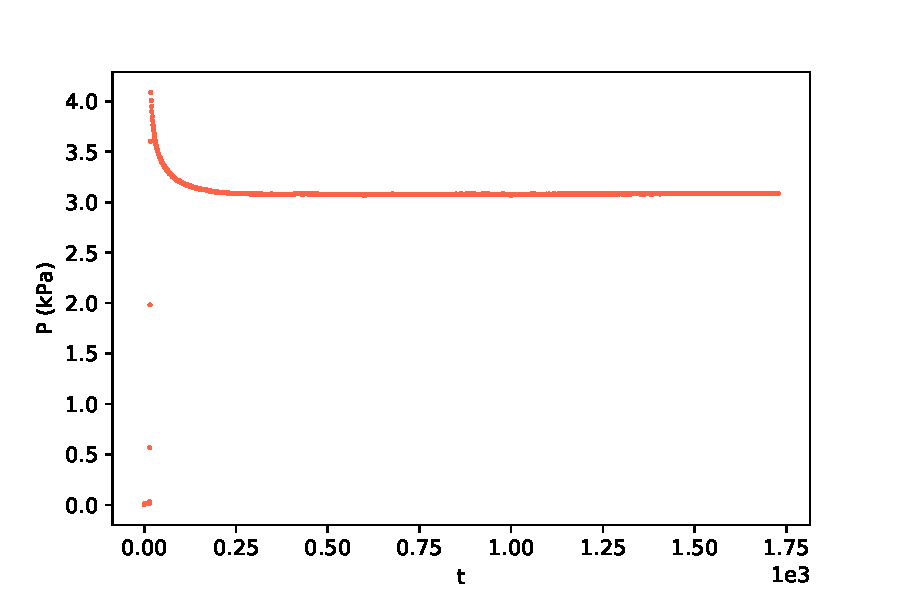
\includegraphics[width=\textwidth]{Pvst-compression.pdf}
\captionof{figure}{Andamento della pressione in funzione del tempo, $\Delta V = \SI{10}{mL}$}
\label{fig:Pvst-compression}
\end{Figure}

%ESPANSIONE
\subsection{Espansione adiabatica dell'aria e successiva termalizzazione isocora}
\label{subsec:expansion}
\paragraph{Situazione reale}


%CURVE SU PIANO P-V
\subsection{Trasformazione adiabatica e isoterma sul piano di Clapeyron}
\label{subsec:clapeyron}
\paragraph{Situazione reale}





%==================================================
%				CONSIDERAZIONI FINALI
%==================================================
\section{Considerazioni finali}


\end{multicols}
\end{document}
